\section{Parameter and source ledger}\label{app:ledger}
Table~\ref{tab:ledger} records, for every parameter that enters the index or the nutrition accounting:
\begin{itemize}
\item its value and exact source location;
\item the experiment behind it;
\item the temperature metric and the outcome measured;
\item whether the value is published, derived by us, or a proxy;
\item the alternatives tested.
\end{itemize}
Verbatim quotes and read levels are in \file{docs/literature\_verification\_new\_crops.md} (new crops, including the
follow-up checks of this audit in its Section~8) and in the mid-evaluation verification notes (original crops).

\paragraph{Read levels.} Full texts were read for:
\begin{itemize}
\item \citet{bhandari2020}, \citet{boote2005}, \citet{tari2022};
\item FAO-33, FAO-66, FAO-56 and FAO-56 Rev.1;
\item WHO/FAO 2004;
\item the Deryng, Yoshida and Jagadish sources.
\end{itemize}
Only abstracts were available for \citet{prasad2002bean}, \citet{prasad2003peanut}, \citet{morrison2002},
\citet{nandi2021} and \citet{istanbulluoglu2010}. The chickpea $K_y$ range 0.67--0.93 attributed to Jalota et al.\
(2006) is known only through a secondary citation; that study's abstract gives no $K_y$.

\paragraph{Derived heat parameters.} The derived thresholds and slopes are refitted from the published data by
\file{code/25\_parameter\_fits.py} (Table~\ref{tab:fits}). The model is the Deryng broken-stick function
$\text{loss} = \min(1, s_T\max(0,\Teff-\Tcrit))$, fitted by least squares on a grid. Chamber day/night regimes
$D/N$ are converted with $\Teff = ((D+N)/2 + D)/2$.

{\scriptsize\begin{longtable}{L{0.091}L{0.098}L{0.098}L{0.171}L{0.183}L{0.140}L{0.122}L{0.098}}
\caption[Parameter and source ledger]{Parameter and source ledger. Values are read from \texttt{code/config.py}. Status: published = value printed in the source; DERIVED = our arithmetic or fit on published values; PROXY = value borrowed from another crop, outcome or metric. Read levels and verbatim quotes: \texttt{docs/literature\_verification\_new\_crops.md}.}\label{tab:ledger}\\
\toprule
Crop & Parameter & Value & Source and location & Experiment / conditions & Metric and outcome & Status & Alternatives tested \\
\midrule\endfirsthead
\toprule
Crop & Parameter & Value & Source and location & Experiment / conditions & Metric and outcome & Status & Alternatives tested \\
\midrule\endhead
\bottomrule\endfoot
Rice & $T_{crit}$ & 35.0 & \citet{yoshida1981} Table 2.4; FAO-66 p.~106 & critical high temperature at anthesis, $>$1 h & daily mean air $T$; spikelet sterility & published (metric differs from $T_{eff}$) & $\pm$1--3\,\si{\celsius} \\
Rice & $s_T$ & 0.070 & \citet{jagadish2007} & IR64 in chambers, $\le$1 h at anthesis & spikelet fertility ($\approx$7\%/\si{\celsius} above 29.6\,\si{\celsius}) & published, outcome borrowed (fertility $\to$ yield) & -- \\
Rice & $K_y$ & 1.25 & FAO-33 Table 2 p.~7 (rice ``high'', no number); maize value FAO-66 Table 1 & -- & seasonal yield--ET response & PROXY (maize) & 1.0, 1.5 \\
Wheat & $T_{crit}$, $T_{lim}$ & 25, 35 & \citet{deryng2014} Table A.1 & PEGASUS model, spring wheat & $T_{eff}$, 45--70\% of season; yield & published model parameter (also used for winter wheat) & $\pm$1--3\,\si{\celsius} \\
Wheat & $K_y$ & 1.10 & FAO-66 Table 1 (spring 1.15, winter 1.05) & -- & seasonal & DERIVED mean of two FAO values & -- \\
Maize & $T_{crit}$, $T_{lim}$ & 32, 45 & \citet{deryng2014} Table A.1 & PEGASUS model & $T_{eff}$; yield & published model parameter & $\pm$1--3\,\si{\celsius} \\
Maize & $K_y$ & 1.25 & FAO-66 Table 1 (= FAO-33) & -- & seasonal & published & -- \\
Soybean & $T_{crit}$, $T_{lim}$ & 35, 40 & \citet{deryng2014} Table A.1 & PEGASUS model & $T_{eff}$; yield & published model parameter & $\pm$1--3\,\si{\celsius} \\
Soybean & $K_y$ & 0.85 & FAO-66 Table 1 (= FAO-33) & -- & seasonal & published & -- \\
Chickpea & $T_{crit}$, $s_T$ & 34.0, 0.140 & \citet{bhandari2020} Table 3 p.~749 & 3 Indian genotypes, pots, growth chambers 30/20--42/32\,\si{\celsius} (12/12 h), flowering to maturity & seed yield per plant & DERIVED fit (5 points) & $T_{crit}$ 30.3 (pod set, \citealp{devasirvatham2013}); +3\,\si{\celsius}; slope $\times$0.7 \\
Chickpea & $K_y$ & 0.88 & \citet{tari2022} p.~143 & field, Konya (Turkey), 2 years, 2 sowing dates & seasonal (0.85, 0.91) & DERIVED mean of 2 field values; not in FAO & 0.67, 1.15 \\
Lentil & $T_{crit}$, $s_T$ & 31.9, 0.170 & \citet{bhandari2020} Table 3 & 2 Indian genotypes, as chickpea & seed yield per plant & DERIVED fit (4 points, 2 parameters) & +3\,\si{\celsius}; slope $\times$0.7 \\
Lentil & $K_y$ & 1.00 & \citet{nandi2021} abstract & field, Lower Gangetic Plain, after rice & ``1\% yield loss per 1\% decline in relative ET''; best treatment 0.87 & PROXY (abstract only) & 0.87, 1.15 \\
Common bean & $T_{crit}$, $s_T$ & 25.5, 0.111 & \citet{prasad2002bean} via \citet{boote2005} p.~470 & cv.\ Montcalm (Andean red kidney), sunlit chambers, season-long, 10\,\si{\celsius} diurnal range & seed yield (max at 28/18, zero at 37/27\,\si{\celsius}) & DERIVED from two published points; full text not read & $T_{crit}$ +2\,\si{\celsius}; slope $\times$0.7 \\
Common bean & $K_y$ & 1.15 & FAO-33 Table 24 p.~39; FAO-66 Table 1 & -- & seasonal (IAEA field 0.59, 1.43) & published & 0.6, 1.4 \\
Groundnut & $T_{crit}$, $s_T$ & 31.8, 0.095 & \citet{prasad2003peanut} abstract & cv.\ Georgia Green, sunlit chambers 32/22--44/34\,\si{\celsius}, season-long, ambient CO$_2$ & seed yield ($-$14, $-$59, $-$90\%) & DERIVED fit (4 points); full text not read & 29.0/0.074 \citep{boote2005}; +3\,\si{\celsius}; slope $\times$0.7 \\
Groundnut & $K_y$ & 0.70 & FAO-33 Table 24; FAO-66 Table 1 & -- & seasonal & published & -- \\
Rapeseed-mustard & $T_{crit}$ & 26.5 & \citet{morrison2002} abstract & field, Ottawa, 3 years $\times$ 3 sowing dates, 3 \emph{Brassica} species incl.\ \emph{B.~juncea} & accumulated daily $T_{\max}$ above 29.5\,\si{\celsius} at flowering; seed yield & PROXY conversion to $T_{eff}$ with an assumed 12\,\si{\celsius} diurnal range & $\pm$1--3\,\si{\celsius} \\
Rapeseed-mustard & $s_T$ & 0.10 & borrowed: \citet{deryng2014} spring-wheat span (10\,\si{\celsius}) & -- & -- & PROXY (no published slope found) & 0.07, 0.18 \\
Rapeseed-mustard & $K_y$ & 0.90 & FAO-56 Rev.1 Table 8.7 p.~279 \citep{fao56rev1} & no source stated by FAO; field 0.87 \citep{istanbulluoglu2010} & seasonal & published, origin not traceable & 0.85, 0.95 \\
Rice & $K_c$ ini, mid, end; $\bar K_c$ & 1.05, 1.20, 0.75; 1.11 & FAO-56 Tables 11--12 \citep{fao56} & subhumid reference conditions & crop water need ($\mathrm{ET_c}=K_c\mathrm{ET_0}$) & published & -- \\
Wheat & $K_c$ ini, mid, end; $\bar K_c$ & 0.40, 1.15, 0.33; 0.88 & FAO-56 Tables 11--12 \citep{fao56} & subhumid reference conditions & crop water need ($\mathrm{ET_c}=K_c\mathrm{ET_0}$) & published & -- \\
Maize & $K_c$ ini, mid, end; $\bar K_c$ & 0.30, 1.20, 0.48; 0.84 & FAO-56 Tables 11--12 \citep{fao56} & subhumid reference conditions & crop water need ($\mathrm{ET_c}=K_c\mathrm{ET_0}$) & published & -- \\
Soybean & $K_c$ ini, mid, end; $\bar K_c$ & 0.40, 1.15, 0.50; 0.89 & FAO-56 Tables 11--12 \citep{fao56} & subhumid reference conditions & crop water need ($\mathrm{ET_c}=K_c\mathrm{ET_0}$) & published & -- \\
Chickpea & $K_c$ ini, mid, end; $\bar K_c$ & 0.40, 1.00, 0.35; 0.77 & FAO-56 Tables 11--12 \citep{fao56}; stages: lentil arid row & subhumid reference conditions & crop water need ($\mathrm{ET_c}=K_c\mathrm{ET_0}$) & published; stages PROXY & -- \\
Lentil & $K_c$ ini, mid, end; $\bar K_c$ & 0.40, 1.10, 0.30; 0.83 & FAO-56 Tables 11--12 \citep{fao56} & subhumid reference conditions & crop water need ($\mathrm{ET_c}=K_c\mathrm{ET_0}$) & published & -- \\
Common bean & $K_c$ ini, mid, end; $\bar K_c$ & 0.40, 1.15, 0.35; 0.85 & FAO-56 Tables 11--12 \citep{fao56} & subhumid reference conditions & crop water need ($\mathrm{ET_c}=K_c\mathrm{ET_0}$) & published & -- \\
Groundnut & $K_c$ ini, mid, end; $\bar K_c$ & 0.40, 1.15, 0.60; 0.85 & FAO-56 Tables 11--12 \citep{fao56} & subhumid reference conditions & crop water need ($\mathrm{ET_c}=K_c\mathrm{ET_0}$) & published & -- \\
Rapeseed-mustard & $K_c$ ini, mid, end; $\bar K_c$ & 0.35, 1.15, 0.35; 0.78 & FAO-56 Tables 11--12 \citep{fao56}; stages: Rev.1 Table 6.11 GDD shares & subhumid reference conditions & crop water need ($\mathrm{ET_c}=K_c\mathrm{ET_0}$) & published; stages PROXY & -- \\
All & Flowering window & 45--70\% of season & \citet{deryng2014} & anthesis at 0.5 of the season & -- & published (model convention) & -- \\
Chickpea, lentil, rapeseed & Calendar & cool-season rule & \citet{sacks2010} (own observed calendar, else wheat/spring-wheat calendar) & Sacks ``Pulses'' calendar is 95\% gap-filled in India and monsoon-season & -- & PROXY (borrowed calendars) & plain Sacks calendar \\
All & $\mathrm{ET_0}$ & Hargreaves & FAO-56 Eq.~52 \citep{fao56} & needs $T_{\max}$, $T_{\min}$, $R_a$ only & -- & published & -- \\
All & Zn requirement & 11.9 mg/d & WHO/FAO 2004 Table 12.4 p.~240 \citep{whofao2004} & adults, low bioavailability (women 9.8, men 14.0) & RNI (upper percentile) & DERIVED mean of two RNIs & 5.95 (moderate) \\
All & Fe requirement & 21.55 mg/d & WHO/FAO 2004 Table 13.5 p.~271 & adults, 10\% bioavailability (women 29.4, men 13.7) & RNI (95th percentile) & DERIVED mean of two RNIs & 14.35 (15\%) \\
All & Energy, protein, fat requirement & ADER; 10\%, 15\% of energy & FAOSTAT food-security indicators; \citet{who2003} & country- and year-specific energy requirement & population average (energy); lower bounds of goals & published & -- \\
All & Zn, Fe composition & per FBS item & USDA SR Legacy \citep{usda2019}; \texttt{code/fbs\_usda\_map.csv} & raw, unprocessed form (whole grain; primary weight) & mg/100 g & mapping choice (overstates Zn, Fe for refined cereals, meat) & -- \\
\end{longtable}}


\begin{table}[H]\centering\small\caption{Derived heat parameters refitted from published data, compared with
\file{config.py} (bean: two published points; rapeseed: converted threshold and borrowed slope).}\label{tab:fits}
\adjustbox{max width=\linewidth}{\begin{tabular}{lp{2.6cm}p{2.6cm}rrrrrc}
\toprule
Crop & $T_{eff}$ points (\si{\celsius}) & relative loss & $T_{crit}$ & $s_T$ & $T_{lim}$ & RMSE & config & match \\
\midrule
Chickpea & 27.5; 32.5; 35.5; 37.5; 39.5 & 0.000; 0.027; 0.219; 0.460; 0.790 & 34.05 & 0.1420 & 41.09 & 0.020 & 34.0 / 0.140 & yes \\
Lentil & 27.5; 32.5; 35.5; 37.5 & 0.000; 0.138; 0.534; 1.000 & 31.85 & 0.1685 & 37.78 & 0.049 & 31.9 / 0.170 & yes \\
Groundnut & 29.5; 33.5; 37.5; 41.5 & 0.000; 0.140; 0.590; 0.900 & 31.75 & 0.0945 & 42.33 & 0.029 & 31.8 / 0.095 & yes \\
Common bean & 25.5; 34.5 & 0; 1 & 25.50 & 0.1111 & 34.50 &  & 25.5 / 0.111 & yes \\
Rapeseed-mustard &  &  & 26.50 & 0.1000 & 36.50 &  & 26.5 / 0.100 & yes \\
\bottomrule
\end{tabular}
}\end{table}

\clearpage
\section{Full result tables}\label{app:tables}

\begin{table}[H]\centering\scriptsize\caption{Country by crop \Fd, 2001--2024.}\label{tab:countrycrop}
\adjustbox{max width=\linewidth}{\begin{minipage}{\textwidth}\centering
\adjustbox{max width=\textwidth}{\begin{tabular}{lrrrrrrrrr}
\toprule
Country & Wheat & Rice & Maize & Chickpea & Lentil & Common bean & Soybean & Groundnut & Rapeseed \\
\midrule
Russia & 0.1315 & -- & -- & 0.0000 & 0.0011 & -- & 0.0036 & -- & -- \\
South Africa & -- & -- & 0.1237 & -- & -- & -- & 0.0137 & -- & $<$0.0001 \\
USA & 0.0903 & $<$0.0001 & 0.0049 & 0.0000 & 0.0003 & 0.0046 & 0.0222 & 0.0017 & 0.0042 \\
India & 0.0676 & 0.0031 & 0.0009 & 0.0273 & 0.0068 & 0.0250 & 0.0002 & 0.0025 & 0.0166 \\
Brazil & 0.0131 & 0.0054 & 0.0137 & -- & -- & 0.0459 & 0.0028 & 0.0005 & $<$0.0001 \\
Tanzania & -- & -- & -- & -- & -- & 0.0357 & -- & -- & -- \\
Ukraine & -- & -- & 0.0332 & -- & -- & -- & -- & -- & -- \\
China & 0.0320 & $<$0.0001 & 0.0016 & 0.0000 & 0.0000 & 0.0004 & 0.0082 & 0.0016 & 0.0018 \\
Canada & -- & -- & -- & -- & 0.0056 & -- & -- & -- & 0.0316 \\
Myanmar & -- & -- & -- & -- & -- & 0.0088 & -- & -- & -- \\
Nigeria & -- & 0.0064 & -- & -- & -- & -- & -- & 0.0012 & -- \\
Australia & -- & -- & -- & 0.0063 & 0.0000 & -- & -- & -- & -- \\
Argentina & -- & -- & -- & -- & -- & -- & 0.0040 & -- & -- \\
Egypt & 0.0036 & -- & -- & -- & -- & -- & -- & -- & -- \\
Turkey & -- & -- & -- & 0.0024 & -- & -- & -- & -- & -- \\
Italy & -- & 0.0015 & -- & -- & -- & -- & -- & -- & -- \\
Ethiopia & -- & -- & -- & 0.0008 & 0.0008 & -- & -- & -- & -- \\
Bangladesh & -- & 0.0003 & -- & -- & -- & -- & -- & -- & -- \\
France & -- & -- & -- & -- & -- & -- & -- & -- & 0.0002 \\
Belarus & -- & -- & -- & -- & -- & $<$0.0001 & -- & -- & -- \\
\bottomrule
\end{tabular}
}
\par\vspace{2pt}{\footnotesize -- = country not in the crop's panel. Values: F4, 2001--2024 stress level, literature-only sensitivity.}
\end{minipage}
}\end{table}

\begin{table}[H]\centering\small\caption{Nutrient adequacy ratios, 2021--23, main and alternative requirements.}\label{tab:adequacy}
\adjustbox{max width=\linewidth}{\begin{tabular}{lrrrrrrrrr}
\toprule
Country & kcal & protein & fat & Zn & Fe & MAR & Zn mod. & Fe 15\% & MAR alt \\
\midrule
Bangladesh & 1.00 & 1.00 & 1.00 & 1.00 & 0.70 & 93.9 & 1.00 & 1.00 & 100.0 \\
South Africa & 1.00 & 1.00 & 1.00 & 1.00 & 0.82 & 96.4 & 1.00 & 1.00 & 100.0 \\
Tanzania & 1.00 & 1.00 & 1.00 & 1.00 & 0.83 & 96.7 & 1.00 & 1.00 & 100.0 \\
Myanmar & 1.00 & 1.00 & 1.00 & 1.00 & 0.89 & 97.7 & 1.00 & 1.00 & 100.0 \\
India & 1.00 & 1.00 & 1.00 & 1.00 & 0.89 & 97.8 & 1.00 & 1.00 & 100.0 \\
Nigeria & 1.00 & 1.00 & 1.00 & 1.00 & 0.91 & 98.1 & 1.00 & 1.00 & 100.0 \\
Brazil & 1.00 & 1.00 & 1.00 & 1.00 & 0.97 & 99.4 & 1.00 & 1.00 & 100.0 \\
Australia & 1.00 & 1.00 & 1.00 & 1.00 & 1.00 & 100.0 & 1.00 & 1.00 & 100.0 \\
Egypt & 1.00 & 1.00 & 1.00 & 1.00 & 1.00 & 100.0 & 1.00 & 1.00 & 100.0 \\
China & 1.00 & 1.00 & 1.00 & 1.00 & 1.00 & 100.0 & 1.00 & 1.00 & 100.0 \\
Canada & 1.00 & 1.00 & 1.00 & 1.00 & 1.00 & 100.0 & 1.00 & 1.00 & 100.0 \\
Belarus & 1.00 & 1.00 & 1.00 & 1.00 & 1.00 & 100.0 & 1.00 & 1.00 & 100.0 \\
Italy & 1.00 & 1.00 & 1.00 & 1.00 & 1.00 & 100.0 & 1.00 & 1.00 & 100.0 \\
France & 1.00 & 1.00 & 1.00 & 1.00 & 1.00 & 100.0 & 1.00 & 1.00 & 100.0 \\
Ethiopia & 1.00 & 1.00 & 1.00 & 1.00 & 1.00 & 100.0 & 1.00 & 1.00 & 100.0 \\
Argentina & 1.00 & 1.00 & 1.00 & 1.00 & 1.00 & 100.0 & 1.00 & 1.00 & 100.0 \\
Russia & 1.00 & 1.00 & 1.00 & 1.00 & 1.00 & 100.0 & 1.00 & 1.00 & 100.0 \\
Turkey & 1.00 & 1.00 & 1.00 & 1.00 & 1.00 & 100.0 & 1.00 & 1.00 & 100.0 \\
Ukraine & 1.00 & 1.00 & 1.00 & 1.00 & 1.00 & 100.0 & 1.00 & 1.00 & 100.0 \\
USA & 1.00 & 1.00 & 1.00 & 1.00 & 1.00 & 100.0 & 1.00 & 1.00 & 100.0 \\
\bottomrule
\end{tabular}
\par\vspace{2pt}{\footnotesize NAR = min(1, national supply / requirement), 2021--23. Main: zinc low bioavailability, iron 10\% bioavailability (WHO/FAO 2004 RNIs). Alternative: moderate zinc, 15\% iron. RNIs are individual upper-percentile requirements compared with national mean supply, so both overstate shortfall.}
}\end{table}

\begin{table}[H]\centering\small\caption{Standard $-10\%$ yield shock: pairs with the largest MAR changes (upper
bound; last column with exports absorbing first).}\label{tab:shock}
\adjustbox{max width=\linewidth}{\begin{minipage}{\textwidth}\centering
\adjustbox{max width=\textwidth}{\begin{tabular}{lrrrrrrrr}
\toprule
Pair & min(1,SSR) & $\Delta$kcal \% & $\Delta$prot \% & $\Delta$Zn \% & $\Delta$Fe \% & MAR & $\Delta$MAR & w/ exports \\
\midrule
Maize--South Africa & 1.00 & -2.17 & -2.20 & -2.95 & -3.23 & 96.4 & -0.53 & -0.00 \\
Wheat--India & 1.00 & -2.11 & -2.38 & -3.26 & -2.95 & 97.8 & -0.52 & -0.28 \\
Rice--Bangladesh & 1.00 & -6.29 & -4.74 & -5.45 & -3.62 & 93.9 & -0.50 & -0.50 \\
Common bean--Tanzania & 1.00 & -0.55 & -1.56 & -0.89 & -1.96 & 96.7 & -0.33 & -0.14 \\
Wheat--Brazil & 0.69 & -0.75 & -0.77 & -1.41 & -1.57 & 99.4 & -0.31 & +0.00 \\
Common bean--Brazil & 1.00 & -0.31 & -0.70 & -0.48 & -1.32 & 99.4 & -0.26 & -0.16 \\
Rice--India & 1.00 & -2.47 & -1.80 & -2.09 & -1.15 & 97.8 & -0.20 & -0.00 \\
Maize--Brazil & 1.00 & -0.72 & -0.50 & -0.92 & -1.05 & 99.4 & -0.20 & +0.00 \\
Groundnut--Nigeria & 0.99 & -0.55 & -0.71 & -0.56 & -0.52 & 98.1 & -0.09 & -0.09 \\
Common bean--India & 0.94 & -0.13 & -0.31 & -0.20 & -0.44 & 97.8 & -0.08 & -0.07 \\
Rice--Brazil & 1.00 & -0.78 & -0.52 & -0.59 & -0.40 & 99.4 & -0.08 & +0.00 \\
Chickpea--India & 1.00 & -0.23 & -0.51 & -0.34 & -0.40 & 97.8 & -0.07 & -0.06 \\
\bottomrule
\end{tabular}
}
\par\vspace{2pt}{\footnotesize Standard $-10\%$ yield shock, no market response; national supply 2021--23. MAR and $\Delta$MAR in points out of 100. 'w/ exports' = exports absorb the loss first.}
\end{minipage}
}\end{table}

\begin{table}[H]\centering\small\caption{Largest future changes by pair, split into heat and water parts.}\label{tab:futurepairs}
\adjustbox{max width=\linewidth}{\begin{minipage}{\textwidth}\centering
\adjustbox{max width=\textwidth}{\begin{tabular}{lrrrrrrr}
\toprule
Pair & 1971--2000 & 2041--60 & $\Delta$F4 & \% & from heat & from water & $\Delta T_{eff}$ \\
\midrule
Wheat--Russia & 0.1286 & 0.1493 & +0.0207 & +16\% & +0.0071 & +0.0136 & +2.5 \\
Common bean--Tanzania & 0.0385 & 0.0574 & +0.0188 & +49\% & +0.0094 & +0.0094 & +1.7 \\
Common bean--Brazil & 0.0409 & 0.0548 & +0.0139 & +34\% & +0.0112 & +0.0026 & +2.1 \\
Wheat--India & 0.0612 & 0.0717 & +0.0105 & +17\% & +0.0102 & +0.0003 & +1.5 \\
Wheat--USA & 0.0894 & 0.0998 & +0.0104 & +12\% & +0.0058 & +0.0046 & +2.4 \\
Maize--Ukraine & 0.0283 & 0.0327 & +0.0044 & +16\% & +0.0000 & +0.0044 & +3.3 \\
Soybean--USA & 0.0259 & 0.0297 & +0.0039 & +15\% & +0.0002 & +0.0037 & +3.1 \\
Wheat--Brazil & 0.0097 & 0.0124 & +0.0027 & +27\% & +0.0005 & +0.0021 & +1.7 \\
\bottomrule
\end{tabular}
}
\par\vspace{2pt}{\footnotesize Largest increases. 'from heat/water' = the change in each hazard term (future sensitivity and importance, fixed).}
\end{minipage}
}\end{table}

\begin{table}[H]\centering\small\caption{Conditional future yield and nutrient change: pairs with the largest MAR
changes (conditional screening estimate).}\label{tab:futnut}
\adjustbox{max width=\linewidth}{\begin{tabular}{lrrrrrr}
\toprule
Pair & $\Delta Y$ lit \% & $\Delta Y$ emp \% & $\Delta$kcal \% & $\Delta$Fe \% & $\Delta$MAR & w/ exports \\
\midrule
Common bean--Brazil & -25.6 & +0.0 & -0.80 & -3.39 & -0.66 & -0.57 \\
Common bean--Tanzania & -17.7 & +0.0 & -0.97 & -3.47 & -0.58 & -0.42 \\
Wheat--India & -4.2 & -6.5 & -0.88 & -1.23 & -0.22 & -0.00 \\
Common bean--India & -17.5 & +0.0 & -0.22 & -0.78 & -0.14 & -0.13 \\
Common bean--Myanmar & -21.5 & +0.0 & -0.19 & -0.74 & -0.13 & -0.00 \\
Maize--Brazil & -2.7 & -18.3 & -0.20 & -0.29 & -0.06 & +0.00 \\
Wheat--Brazil & -1.7 & -3.0 & -0.13 & -0.27 & -0.05 & +0.00 \\
Rice--Brazil & -0.8 & +0.0 & -0.06 & -0.03 & -0.01 & +0.00 \\
Groundnut--Brazil & -9.7 & -3.6 & -0.01 & -0.02 & -0.00 & +0.00 \\
Lentil--India & -2.0 & -0.6 & -0.01 & -0.02 & -0.00 & -0.00 \\
\bottomrule
\end{tabular}
\par\vspace{2pt}{\footnotesize Conditional screening estimate: change in climate-attributable loss (heat: $s_T \cdot$ \si{\celsius} above $T_{crit}$; water: $K_y \cdot$ rainfed deficit), 2041--60 vs 1971--2000, MRI-ESM2-0 SSP2-4.5; no CO$_2$ fertilisation, adaptation or market response. Only losses propagated.}
}\end{table}

\begin{table}[H]\centering\scriptsize\caption{One-at-a-time robustness tests (F4).}\label{tab:robust}
\adjustbox{max width=\linewidth}{\begin{tabular}{p{6.8cm}p{5.2cm}cc}
\toprule
Test (one at a time) & Top three, F4 equal weights & Wheat rank eq & rank pw \\
\midrule
main (x/max, exposure = stress level, literature S) & Wheat $>$ Maize $>$ Commo \ldots & 1 & 1 \\
min-max normalisation & Wheat $>$ Maize $>$ Commo \ldots & 1 & 1 \\
exposure = level + change (average) & Wheat $>$ Maize $>$ Rice \ldots & 1 & 1 \\
exposure = change only & Wheat $>$ Maize $>$ Rice \ldots & 1 & 1 \\
sensitivity = literature + empirical average (mid-evaluation configuration) & Wheat $>$ Maize $>$ Commo \ldots & 1 & 1 \\
sensitivity = empirical only & Soybe $>$ Lenti $>$ Wheat \ldots & 3 & 3 \\
rice Ky = 1.0 & Wheat $>$ Maize $>$ Commo \ldots & 1 & 1 \\
rice Ky = 1.5 & Wheat $>$ Maize $>$ Commo \ldots & 1 & 1 \\
importance = kcal share only & Wheat $>$ Maize $>$ Soybe \ldots & 1 & 1 \\
importance = Zn+Fe+protein only & Wheat $>$ Maize $>$ Commo \ldots & 1 & 1 \\
heat threshold T crit -2 C (all crops) & Wheat $>$ Maize $>$ Commo \ldots & 1 & 1 \\
heat threshold T crit -1 C (all crops) & Wheat $>$ Maize $>$ Commo \ldots & 1 & 1 \\
heat threshold T crit +1 C (all crops) & Wheat $>$ Maize $>$ Commo \ldots & 1 & 1 \\
heat threshold T crit +2 C (all crops) & Wheat $>$ Maize $>$ Commo \ldots & 1 & 1 \\
heat threshold T crit +3 C (all crops) & Wheat $>$ Maize $>$ Commo \ldots & 1 & 1 \\
new legumes T crit +3 C (chamber vs model thresholds) & Wheat $>$ Maize $>$ Commo \ldots & 1 & 1 \\
bean T crit +2 C (Mesoamerican types) & Wheat $>$ Maize $>$ Commo \ldots & 1 & 1 \\
calendar = plain Sacks (Pulses / Rapeseed.Winter) for chickpea, lentil, rapeseed & Wheat $>$ Maize $>$ Commo \ldots & 1 & 1 \\
new legumes: heat slope x0.7 (chamber -> field) & Wheat $>$ Maize $>$ Commo \ldots & 1 & 1 \\
rapeseed heat slope 0.07 (proxy low) & Wheat $>$ Maize $>$ Commo \ldots & 1 & 1 \\
rapeseed heat slope 0.18 (proxy high) & Wheat $>$ Maize $>$ Commo \ldots & 1 & 1 \\
new crops K y low (chickpea 0.67, lentil 0.87, bean 0.6, rapeseed 0.85) & Wheat $>$ Maize $>$ Commo \ldots & 1 & 1 \\
new crops K y high (chickpea 1.15, lentil 1.15, bean 1.4, rapeseed 0.95) & Wheat $>$ Maize $>$ Commo \ldots & 1 & 1 \\
\bottomrule
\end{tabular}
}\end{table}

\begin{figure}[H]\centering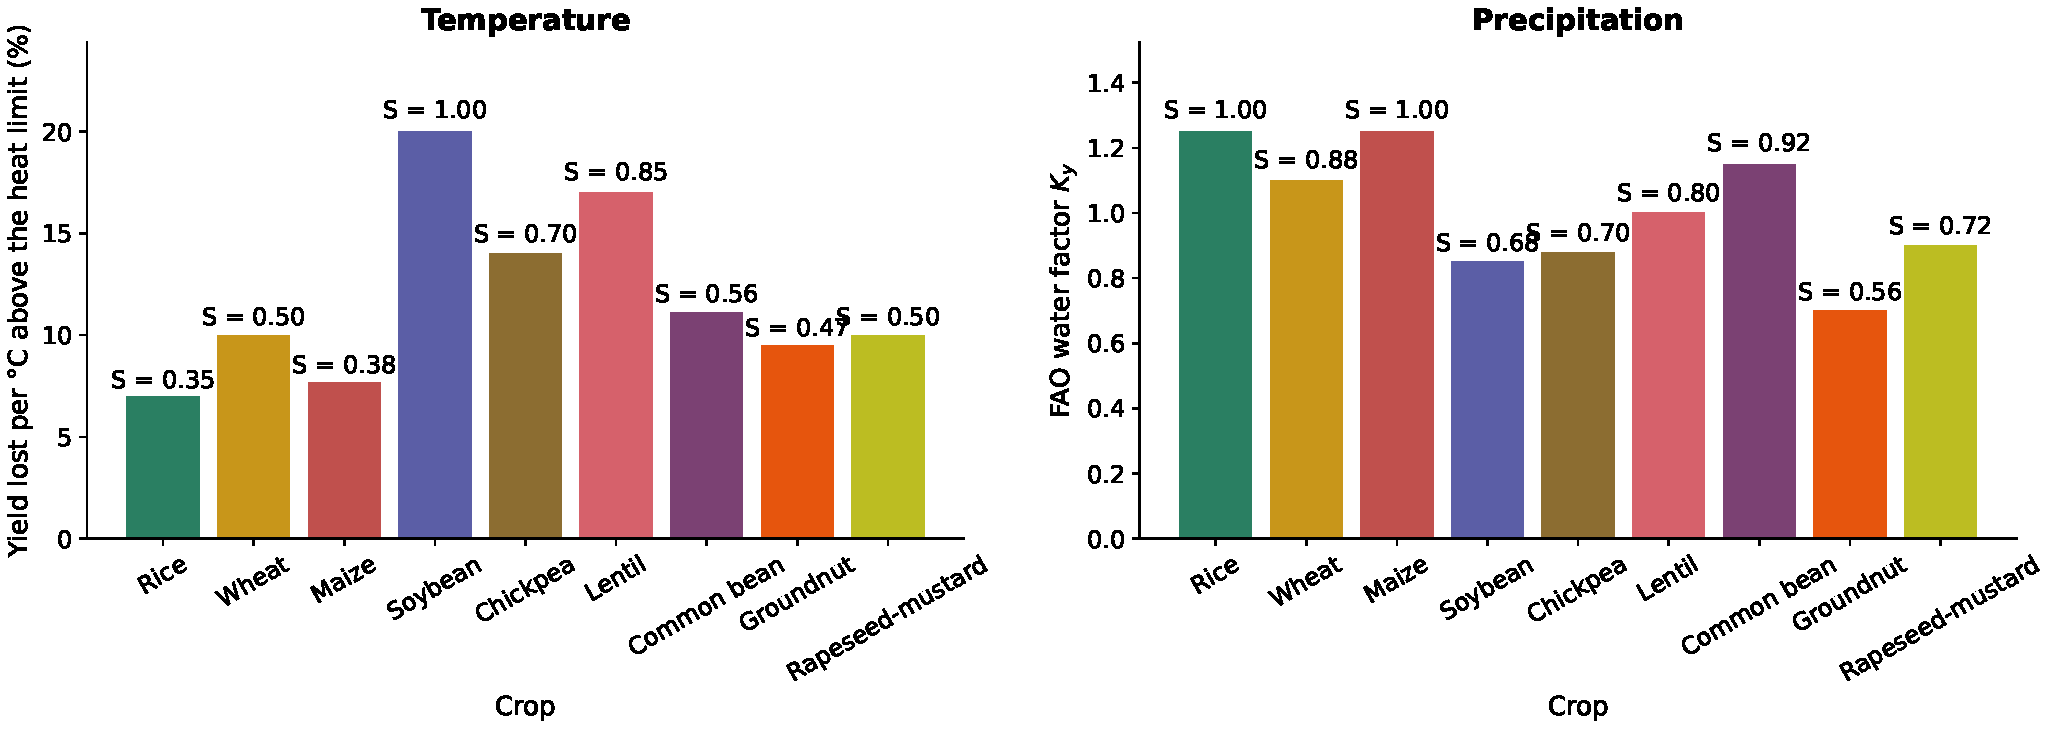
\includegraphics[width=0.85\linewidth]{F05l_literature_sensitivity.pdf}
\caption{Literature sensitivity of the nine crops: heat slope and $K_y$.}\label{fig:litsens}\end{figure}

\begin{figure}[H]\centering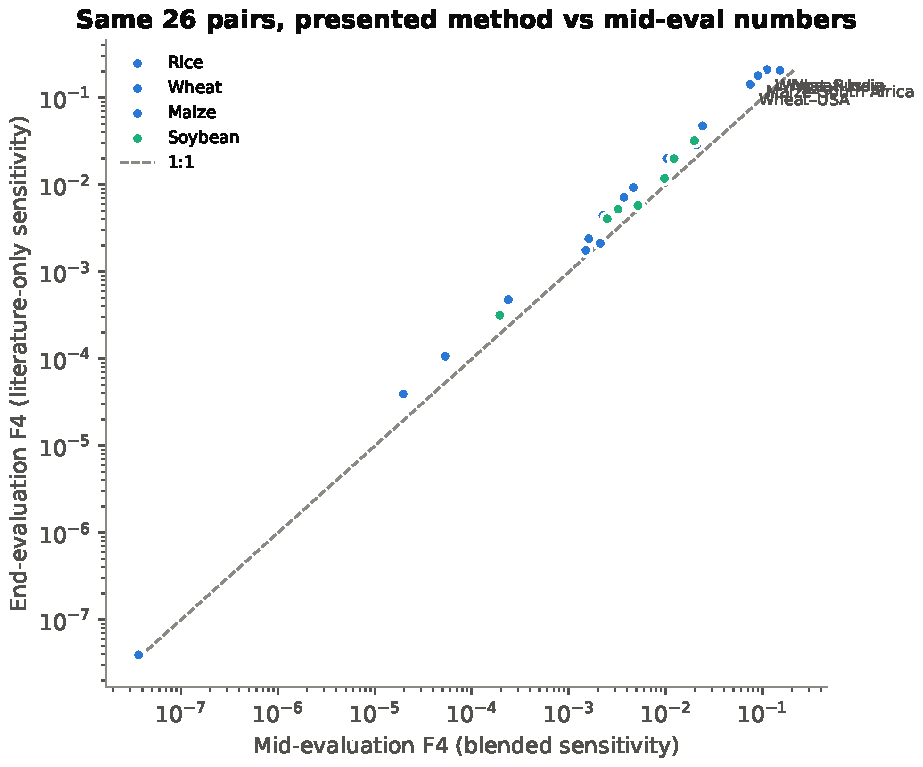
\includegraphics[width=0.6\linewidth]{G11_mideval_vs_literature_only.pdf}
\caption{The same 26 pairs: frozen mid-evaluation values (blended sensitivity) against the presented
literature-only method.}\label{fig:midlit}\end{figure}

\begin{table}[H]\centering\small\caption{Food-supply diversity (effective number of FBS items supplying each
nutrient, 2021--23) and share of supply from the nine crops.}\label{tab:diversity}
\adjustbox{max width=\linewidth}{\begin{tabular}{lrrrrrlrr}
\toprule
Country & kcal & protein & Zn & Fe & cereal \% kcal & top iron source & 9 crops \% kcal & 9 crops \% Fe \\
\midrule
Bangladesh & 5.9 & 8.0 & 6.9 & 10.7 & 68 & Rice and products & 74 & 53 \\
Myanmar & 8.0 & 10.2 & 8.6 & 13.5 & 62 & Rice and products & 70 & 47 \\
Egypt & 12.1 & 10.8 & 7.5 & 8.8 & 62 & Wheat and products & 65 & 68 \\
Ethiopia & 14.0 & 12.1 & 10.8 & 12.1 & 54 & Wheat and products & 43 & 46 \\
India & 16.1 & 12.8 & 11.6 & 13.8 & 51 & Wheat and products & 58 & 56 \\
Russian Federation & 16.8 & 12.5 & 10.1 & 10.2 & 33 & Wheat and products & 33 & 51 \\
South Africa & 16.9 & 11.6 & 9.8 & 10.2 & 43 & Maize and products & 48 & 65 \\
United Republic of Tanzania & 17.0 & 15.5 & 12.6 & 12.4 & 45 & Maize and products & 51 & 67 \\
Türkiye & 17.4 & 11.9 & 9.7 & 11.5 & 37 & Wheat and products & 40 & 53 \\
Ukraine & 17.6 & 13.7 & 11.3 & 11.0 & 34 & Wheat and products & 32 & 46 \\
Argentina & 17.9 & 11.7 & 9.7 & 11.2 & 31 & Wheat and products & 35 & 54 \\
China, mainland & 19.1 & 16.6 & 15.1 & 14.2 & 46 & Vegetables, other & 52 & 39 \\
Nigeria & 19.6 & 19.8 & 17.1 & 17.7 & 37 & Sorghum and products & 33 & 34 \\
Italy & 20.8 & 12.9 & 10.5 & 12.0 & 28 & Wheat and products & 32 & 49 \\
United States of America & 22.6 & 13.5 & 14.6 & 18.1 & 21 & Wheat and products & 37 & 40 \\
Brazil & 22.8 & 13.4 & 13.9 & 16.5 & 27 & Wheat and products & 39 & 51 \\
Belarus & 23.0 & 14.4 & 14.4 & 14.4 & 24 & Wheat and products & 21 & 28 \\
France & 23.8 & 13.9 & 13.3 & 15.3 & 26 & Wheat and products & 29 & 43 \\
Australia & 24.8 & 15.9 & 14.8 & 17.1 & 20 & Wheat and products & 31 & 39 \\
Canada & 25.4 & 17.3 & 16.2 & 18.9 & 24 & Wheat and products & 36 & 44 \\
World & 26.9 & 20.8 & 18.3 & 21.2 & 42 & Wheat and products & -- & -- \\
\bottomrule
\end{tabular}
}\end{table}

\clearpage
\section{Record of corrections}\label{app:corrections}
Table~\ref{tab:corrections} lists every error found after the first end-evaluation version and how it was fixed.
Decisions E18 and E19 are recorded in \file{docs/DECISION\_REGISTER\_END\_EVAL.md}.

{\small
\begin{longtable}{p{0.4cm}p{4.6cm}p{5.0cm}p{4.6cm}}
\caption{Corrections made during the end-evaluation audits.}\label{tab:corrections}\\
\toprule
& Issue & Fix & Effect on results \\
\midrule\endfirsthead
\toprule & Issue & Fix & Effect on results \\ \midrule\endhead
\bottomrule\endfoot
1 & The nine-crop supply share counted only crops with an FBS item of their own, omitting chickpea and lentil. & Numerator from summed crop contributions (SUA for chickpea and lentil), denominator FBS total; World left blank (no SUA); not added to totals or to the Shannon items (E18). & India: energy \shareOldKcal\ $\to$ \shareNewKcal\%, protein \shareOldProtein\ $\to$ \shareNewProtein\%, iron \shareOldIron\ $\to$ \shareNewIron\%, zinc \shareOldZinc\ $\to$ \shareNewZinc\%. No index value changes. \\
2 & Yield-to-nutrient bounds: Canada lentil has negative 2023 domestic supply in FAOSTAT (residuals $-$267\,kt), so SSR $<0$ turned a loss into a gain; in five pairs the lower bound exceeded the upper. & SSR capped to [0,1], non-positive supply with positive production counted as SSR = 1, lower bound $\le$ upper bound, in both historical and future accounting (E19). & 7 historical scenario rows and 3 future rows changed by at most 0.26 percentage points of a nutrient; no ranking or headline value changed. \\
3 & Committed four-crop outputs (empirical sensitivity, S1/S2 scenarios) were stale, i.e.\ not what the code produces. & Regenerated; now identical to the nine-crop run on the 24 shared pairs. & Empirical water slope differed by up to 33, S1/S2 yield changes by up to 20 points; checks only, so no main index value changed. \\
4 & Derived heat parameters were fitted in an unsaved scratch script. & \file{code/25\_parameter\_fits.py} refits them from the tabulated published data (a bounded optimiser hit local minima; replaced by a grid). & Reproduces \file{config.py} to its rounding; no value changed. \\
5 & The raw-data manifest did not list the 19 Telangana-mask and Indian survey files used by the analysis. & Added with checksums, existing rows unchanged. & None. \\
6 & The pipeline did not stop on a failed document compile; no automated arithmetic checks. & Compile exit codes checked; \file{24\_checks.py} runs before the documents. & None. \\
7 & Text said wheat's future increase in the USA is water-driven, and bean has no empirical response in ``most'' countries. & Checked against \file{future\_components.csv} and \file{future\_yield.csv}: USA is shared heat/water; bean has no detected response in any country. & Wording only. \\
8 & Rice $K_y$: FAO-33's rice chapter is at p.~125 and gives no number (rice is classed ``high''). & Proxy label made explicit. & None. \\
9 & Reference: Beach et al.\ (2019) had been cited as ``Smith and Myers 2019''. & Corrected in \file{refs.bib}. & Reference [16] of the submitted literature review still carries the wrong authorship. \\
10 & Layout: a future table ran 174\,pt past the margin; notes shrank tables; overlapping tick labels in a figure. & Tables wrapped and notes set under the table; tick formatter fixed. & None. \\
\end{longtable}}

\clearpage
\section{Audit evidence}\label{app:audit}
{\scriptsize\begin{longtable}{rL{0.569}cL{0.261}}
\caption[Consistency checks run on the saved results]{Consistency checks run on the saved results.}\label{tab:checks}\\
\toprule
 & Check (\texttt{code/24\_checks.py}) & Result & Detail \\
\midrule\endfirsthead
\toprule
 & Check (\texttt{code/24\_checks.py}) & Result & Detail \\
\midrule\endhead
\bottomrule\endfoot
1 & nine crops in panels & pass & 9 crops, 59 pairs \\
2 & every crop appears in docs/input\_register.csv & pass & [] \\
3 & E\_heat = observed level / fixed maximum & pass & max 5.0463 \\
4 & E\_water = observed level / fixed maximum & pass & max 0.7894 \\
5 & index\_reference maxima equal component maxima & pass &  \\
6 & S\_heat is literature slope / max slope (literature-only) & pass &  \\
7 & S\_water is FAO K\_y / max K\_y (literature-only) & pass &  \\
8 & I = mean of five nutrient shares & pass &  \\
9 & In = I / max I & pass &  \\
10 & F4 recomputed from components & pass &  \\
11 & crop score, equal weights = mean over countries & pass &  \\
12 & crop score, production weights & pass &  \\
13 & group score = simple mean of its three crop scores & pass &  \\
14 & future run's 'present' column reproduces the main F4 & pass &  \\
15 & historical\_1971\_2000: E uses the FIXED present-period maximum & pass &  \\
16 & future\_2041\_2060: E uses the FIXED present-period maximum & pass &  \\
17 & S and In identical across periods & pass &  \\
18 & dF4 = heat part + water part & pass &  \\
19 & 1971-2000 comparator reproduces main series (relative < 1e-3) & pass & max rel 1.94e-07 \\
20 & yield change comes from loss accounting, not from index values & pass &  \\
21 & crop\_contrib national totals equal the adequacy (FBS) totals & pass & 2848 country-years \\
22 & nine crops never exceed 100\% of any national nutrient supply & pass & max 0.835 \\
23 & SUA chickpea+lentil kcal do not exceed the FBS 'Pulses, Other' aggregate (5\% tolerance) & pass & 0.1\% of 2369 country-years exceed (SUA and FBS can differ) \\
24 & SUA rows are labelled and kept out of national totals & pass &  \\
25 & India nine-crop share (diversity table) = summed crop contributions & pass & kcal 0.5800 vs 0.5800 \\
26 & nine-crop share >= FBS-item-only share everywhere it is defined & pass &  \\
27 & standard shock is -10\% everywhere & pass &  \\
28 & historical scenarios: supply changes are <= 0 and the lower bound is no larger than the upper bound & pass &  \\
29 & future nutrition: supply changes are <= 0 and the lower bound is no larger than the upper bound & pass &  \\
\end{longtable}}


{\scriptsize\begin{longtable}{L{0.250}L{0.381}L{0.113}rrr}
\caption[Outputs that are not identical in both runs: new outputs of this audit, and previous files the pipeline no longer writes]{Outputs that are not identical in both runs: new outputs of this audit, and previous files the pipeline no longer writes. No file present in both runs differs.}\label{tab:auditdiff}\\
\toprule
Area & File (* = each crop) & Status & Files & max abs & max rel \\
\midrule\endfirsthead
\toprule
Area & File (* = each crop) & Status & Files & max abs & max rel \\
\midrule\endhead
\bottomrule\endfoot
\file{work} & \file{\_qcl\_prod\_2020\_24.pkl} & missing & 1 &  &  \\
\file{work} & \file{\_sua\_pulses.pkl} & missing & 1 &  &  \\
\file{work} & \file{metrics\_prec\_*\_annual.npz} & missing & 12 &  &  \\
\file{work} & \file{metrics\_prec\_*\_flow.npz} & missing & 12 &  &  \\
\file{work} & \file{metrics\_prec\_*\_gs.npz} & missing & 12 &  &  \\
\file{work} & \file{metrics\_tmax\_*\_annual.npz} & missing & 12 &  &  \\
\file{work} & \file{metrics\_tmax\_*\_flow.npz} & missing & 12 &  &  \\
\file{work} & \file{metrics\_tmax\_*\_gs.npz} & missing & 12 &  &  \\
\file{work} & \file{run\_chain.sh} & missing & 1 &  &  \\
\file{processed} & \file{nine\_crop/parameter\_fits.csv} & new & 1 &  &  \\
\file{docs/nine\_crop/generated} & \file{numbers\_report.tex} & new & 1 &  &  \\
\file{docs/nine\_crop/generated} & \file{tab\_audit\_diff.tex} & new & 1 &  &  \\
\file{docs/nine\_crop/generated} & \file{tab\_audit\_summary.tex} & new & 1 &  &  \\
\file{docs/nine\_crop/generated} & \file{tab\_checks.tex} & new & 1 &  &  \\
\file{docs/nine\_crop/generated} & \file{tab\_crop\_mapping.tex} & new & 1 &  &  \\
\file{docs/nine\_crop/generated} & \file{tab\_data\_sources.tex} & new & 1 &  &  \\
\file{docs/nine\_crop/generated} & \file{tab\_diversity.tex} & new & 1 &  &  \\
\file{docs/nine\_crop/generated} & \file{tab\_fits.tex} & new & 1 &  &  \\
\file{docs/nine\_crop/generated} & \file{tab\_india\_shares.tex} & new & 1 &  &  \\
\file{docs/nine\_crop/generated} & \file{tab\_india\_sources.tex} & new & 1 &  &  \\
\file{docs/nine\_crop/generated} & \file{tab\_ledger.tex} & new & 1 &  &  \\
\end{longtable}}


\section{India, Telangana and Hyderabad sources}\label{app:indiasources}
Every number used in Section~\ref{sec:india} is stored once with its table or page in
\file{data/external/india\_hyderabad\_indicators.csv}. The source register \file{docs/india\_hyderabad\_sources.md} is
generated from that file. Table~\ref{tab:indiasources} summarises it.

{\scriptsize\begin{longtable}{L{0.140}L{0.343}L{0.330}rL{0.102}}
\caption[Official sources of the India/Telangana/Hyderabad analysis]{Official sources of the India/Telangana/Hyderabad analysis (from \texttt{data/external/india\_hyderabad\_indicators.csv}).}\label{tab:indiasources}\\
\toprule
Source & Citation & Granularity and use & Rows & Read level \\
\midrule\endfirsthead
\toprule
Source & Citation & Granularity and use & Rows & Read level \\
\midrule\endhead
\bottomrule\endfoot
\file{NFHS5\_TG\_FS} & IIPS \& ICF (2020/2021). National Family Health Survey (NFHS-5) 2019-21, State Fact Sheet: Telangana (Key Indicators). Mumbai: IIPS; Ministry of Health and Family Welfare, Govt of India. & NFHS-5 Telangana state fact sheet (urban, rural, total; NFHS-4 for trend). & 76 & table read \\
\file{NFHS5\_IN\_FS} & IIPS \& ICF (2020). National Family Health Survey (NFHS)-5, India and State Factsheet Compendium (Phase II). Mumbai: IIPS. & NFHS-5 India key indicators (comparison). & 76 & table read \\
\file{NFHS5\_TG\_REP} & International Institute for Population Sciences (IIPS) and ICF. 2021. National Family Health Survey (NFHS-5), India, 2019-21: Telangana. Mumbai: IIPS. & NFHS-5 Telangana state report: food-frequency tables for women and men 15-49, child feeding, anaemia. & 101 & table read \\
\file{NFHS5\_HYD\_DFS} & IIPS / MoHFW. India Districts Factsheets of National Family Health Survey (NFHS)-5, 2019-2021 (district fact sheet values), published on Open Government Data Platform India (data.gov.in), resource cf80173e-fece-439d-a0b1-6e9cb510593d; record District=Hyderabad, State=Telangana. & NFHS-5 Hyderabad DISTRICT fact sheet (fully urban) via the official data.gov.in API. Values printed in parentheses or as * in the source are small-sample and are not used. & 17 & table read (official open-data copy of district fact sheet) \\
\file{CNNS\_TG\_FS} & Ministry of Health and Family Welfare (MoHFW), UNICEF and Population Council. 2019. Comprehensive National Nutrition Survey (CNNS) 2016-18, Telangana Factsheet. New Delhi. & CNNS 2016-18 Telangana fact sheet: serum ferritin, zinc, anaemia, vitamins (children 1-4, 5-9, adolescents 10-19). & 55 & table read \\
\file{CNNS\_NAT} & Ministry of Health and Family Welfare (MoHFW), Government of India, UNICEF and Population Council. 2019. Comprehensive National Nutrition Survey (CNNS) National Report. New Delhi. & CNNS 2016-18 national report tables. & 92 & table read, table read (text layer), table read (text layer, verified against page image for Table 4.5) \\
\file{NSS594} & National Statistics Office, MoSPI, Govt of India. 2025. Nutritional Intake in India (2022-23 \& 2023-24), NSS Report No. 594 (HCES: 2022-23 \& 2023-24). & State x rural/urban nutrient intake (energy, protein, fat) and food-group shares, 2022-23 and 2023-24. & 112 & table read \\
\file{NSS592} & National Statistics Office, MoSPI, Govt of India. 2025. Survey on Household Consumption Expenditure: 2023-24, NSS Report No. 592 (HCES: 2023-24). & State x rural/urban HCES 2023-24 report tables (expenditure shares). & 64 & table read \\
\file{HCES2324\_A10S} & National Statistics Office, MoSPI. HCES 2023-24 (NSS Report No. 592), Appendix Table A10S: Monthly per capita quantity and value of consumption at detailed item level for all items of consumption by State/UT and All-India (Excel). & State x rural/urban household consumption (quantity and value per person per 30 days). Not city-level: Telangana urban is the nearest description of Hyderabad. & 465 & table read \\
\file{TG\_DES\_AAG2024} & Directorate of Economics and Statistics, Government of Telangana. 2024. Telangana State At A Glance 2024. Hyderabad. & Telangana Directorate of Economics and Statistics, At a Glance 2024: crop area and production 2023-24 (provisional), rainfall. & 108 & table read \\
\file{TG\_SEO2025} & Planning Department, Government of Telangana. 2025. Telangana Socio Economic Outlook 2025 (data source: Directorate of Economics and Statistics, Telangana). & Telangana Socio-Economic Outlook 2025: yields, rainfall, net area sown. & 41 & figure data labels read, table read \\
\file{NNMB\_URBAN} & National Nutrition Monitoring Bureau (NNMB), ICMR-National Institute of Nutrition. 2017. Diet and Nutritional Status of Urban Population in India and Prevalence of Obesity, Hypertension, Diabetes and Hyperlipidemia in Urban Men and Women - A brief NNMB Urban Nutrition Report. Hyderabad: NIN. & ICMR-NIN NNMB urban brief report: pooled urban India (16 states); Telangana is NOT included, so it is not used for Hyderabad. & 18 & figure data labels read (scanned report) \\
\file{IFCT2017} & Longvah, T., Ananthan, R., Bhaskarachary, K. and Venkaiah, K. (2017). Indian Food Composition Tables 2017. National Institute of Nutrition (ICMR), Hyderabad, Telangana, India. & ICMR-NIN Indian Food Composition Tables 2017, Table 5 (iron, zinc; mg per 100 g edible portion, raw foods). & 44 & table read \\
\end{longtable}}

